%%% Magic comments for setting the correct parameters in compatible IDEs
% !TeX encoding = utf8
% !TeX program = pdflatex 
% !TeX spellcheck = en_US
% !BIB program = biber

\documentclass[english,notitlepage,smartquotes]{hgbreport}
%%%-----------------------------------------------------------------------------

\RequirePackage[utf8]{inputenc} % Remove when using lualatex or xelatex!

\graphicspath{{images/}}  % Location of images and graphics
\bibliography{references} % Biblatex bibliography file (references.bib)

%%%-----------------------------------------------------------------------------
\begin{document}
%%%-----------------------------------------------------------------------------

\author{Alexander Gärtner, Felix Rader}                    
\title{ AI time machine based on stable diffusion }	                 
\date{\today}

%%%-----------------------------------------------------------------------------
\maketitle
%%%-----------------------------------------------------------------------------

\begin{abstract}\noindent
	This projects investigates the potential of AI tools to generate images of the past. The goal was to create a pipeline that allows for generating images of the past based on a given input image. The pipeline is based on stable diffusion, a recent AI tool that allows for generating images based on a given prompt. Implemented via a web based UI the pipeline allows for uploading images and converting them into past version of themselves 
\end{abstract}

%%%-----------------------------------------------------------------------------
\tableofcontents
%%%-----------------------------------------------------------------------------

%%%-----------------------------------------------------------------------------
\chapter{Aims and Context}
%%%-----------------------------------------------------------------------------

Imagine the potential of future AR devices for tourism: One could walk through a city like Vienna with AR glasses and get a fully modified view of any past reality. For example, one could use a "Time Machine Slider" to see the city 200 years back from now. This would mean that an AI system would take the live feed of the camera and adjust it accordingly - people would wear clothing from previous times, cars would be substituted with horse carriages, advertisements would hint to past events instead of upcoming concerts.  

The purpose of this project was to do a first step towards this vision by investigating recent AI tools and their potential to modify images in a way that they plausibly depict the past. Instead of using video streams,  single images were used and modified by stable diffusion to serve as a starting point.


%%%-----------------------------------------------------------------------------
\chapter{Project Details}
%%%-----------------------------------------------------------------------------

Since no similar previous work exists, as a first step a general pipeline for transforming images to a "past" version of the image had to be developed. Stable diffusion allows for inputting prompts in addition to an image to further shape the outcome of the transformed image. The stable diffusion webUI \cite{webui}, an open-source project which allows for locally hosting a web based UI to interact with a stable diffusion model, served as a basis for researching how to generate "past" images.

In addition to the whole image generation, certain limitation had to be taken into consideration as well. For example, it was important to limit how far back in time the images should be generated in. Since stable diffusion is trained on actual photographs, paintings and so on it naturally has less training data to work with depending on how far back in time one goes. Therefore, the year 1880 was deemed as a reasonable cut-off for the time machine as this was the year photography started to become more common. After a month of research a pipeline for the image generation was developed as can be seen in figure \ref{fig:simpPipeline}.

\begin{figure}[htbp]
    \centering\small
    {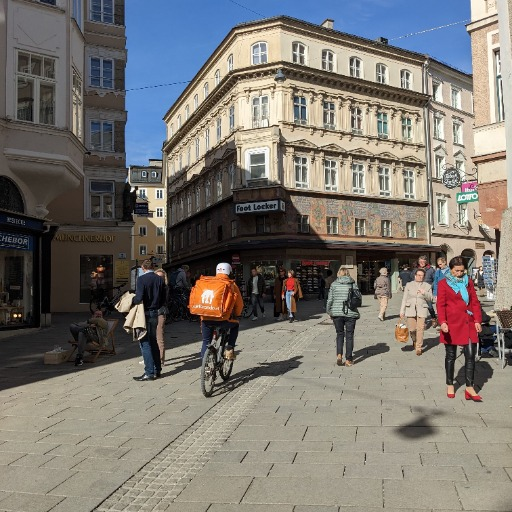
\includegraphics[width=0.8\textwidth]{images/base_image_Salzburg.jpg}}
    \caption{pic of pipeline}
    \label{fig:simpPipeline}
\end{figure}

The pipeline goes as follows:
\begin{enumerate}
    \item Upload Image
    \item resize image to 512x512 which is the preferred format for stable diffusion
    \item if available: read coordinates from image data and assign city and country
    \item set desired past year between 1880 - 2013
    \item interrogate image via stable diffusion to generate base prompt
    \item combine year, geolocation and base prompt into a single prompt
    \item if the year is below 1950 filter out all colors from the prompt and set colors to negative prompt to ensure a black and white image
    \item send prompt to chatGPT and let it filter out objects from the prompt which did not exist in the specified year
    \item add year specific information to filtered prompt like common cameras and techniques
    \item send image and prompt to stable diffusion 
    \item generate canny edges via ControlNet plugin for stable diffusion
    \item generate past image based on prompt and canny edges version of image
    \item output generated image
\end{enumerate}

Based on the pipeline, a simple frontend based on React and NextJS was developed as can be seen in figure \ref{fig:frontendPre}. The frontend implements everything that is needed for uploading and resizing the image. Additionally, it also contains a repertoire of base prompts based on each year. These base prompts contain standard information for each year like which camera was typically used for the time span. Image interrogation and image generation are handled in the background via the stable diffusion webUI to which the frontend makes API calls.
When both the stable diffusion webUI and the web based frontend are locally hosted on a machine it is possible to upload images to the frontend to generate a new image based on a selected year or a GIF based on the whole year range.

\begin{figure}[htbp]
    \centering\small
    {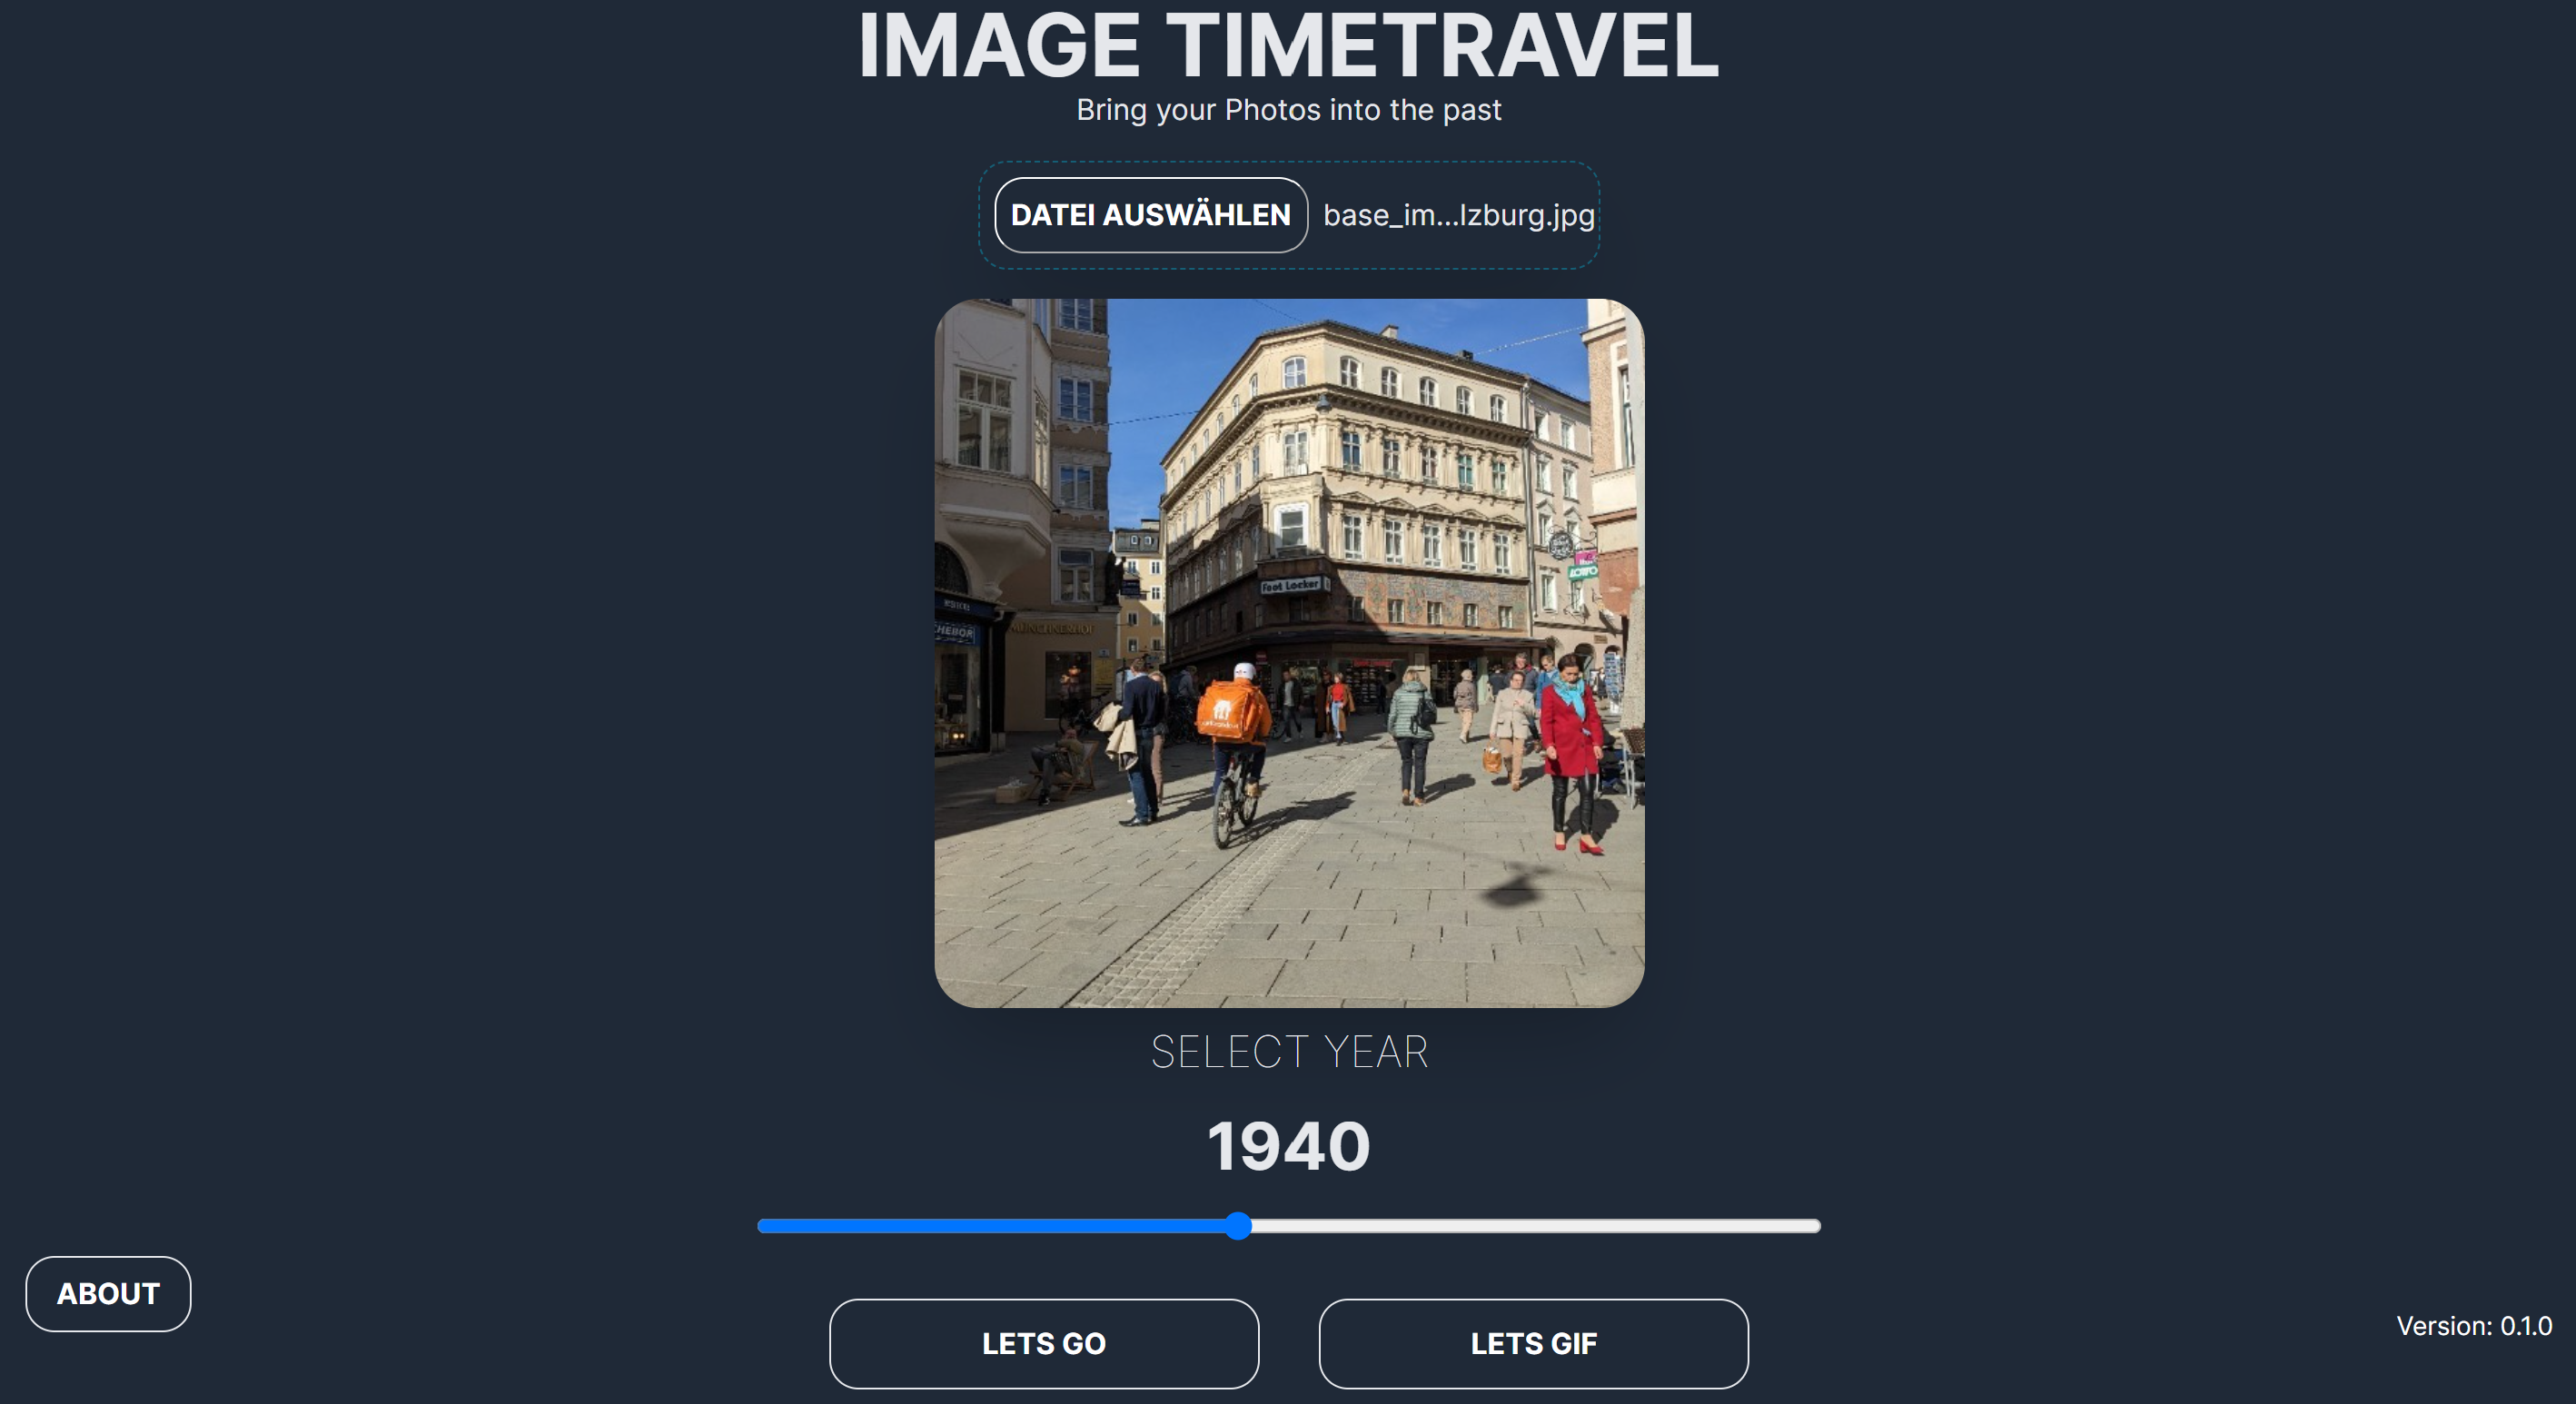
\includegraphics[width=0.8\textwidth]{images/frontendPre.png}}
    \caption{A screenshot of the developed frontend for the time machine. The picture selected is a photograph of a street in Salzburg, Austria taken on a mobile phone}
    \label{fig:frontendPre}
\end{figure}

\begin{figure}[htbp]
    \centering\small
    {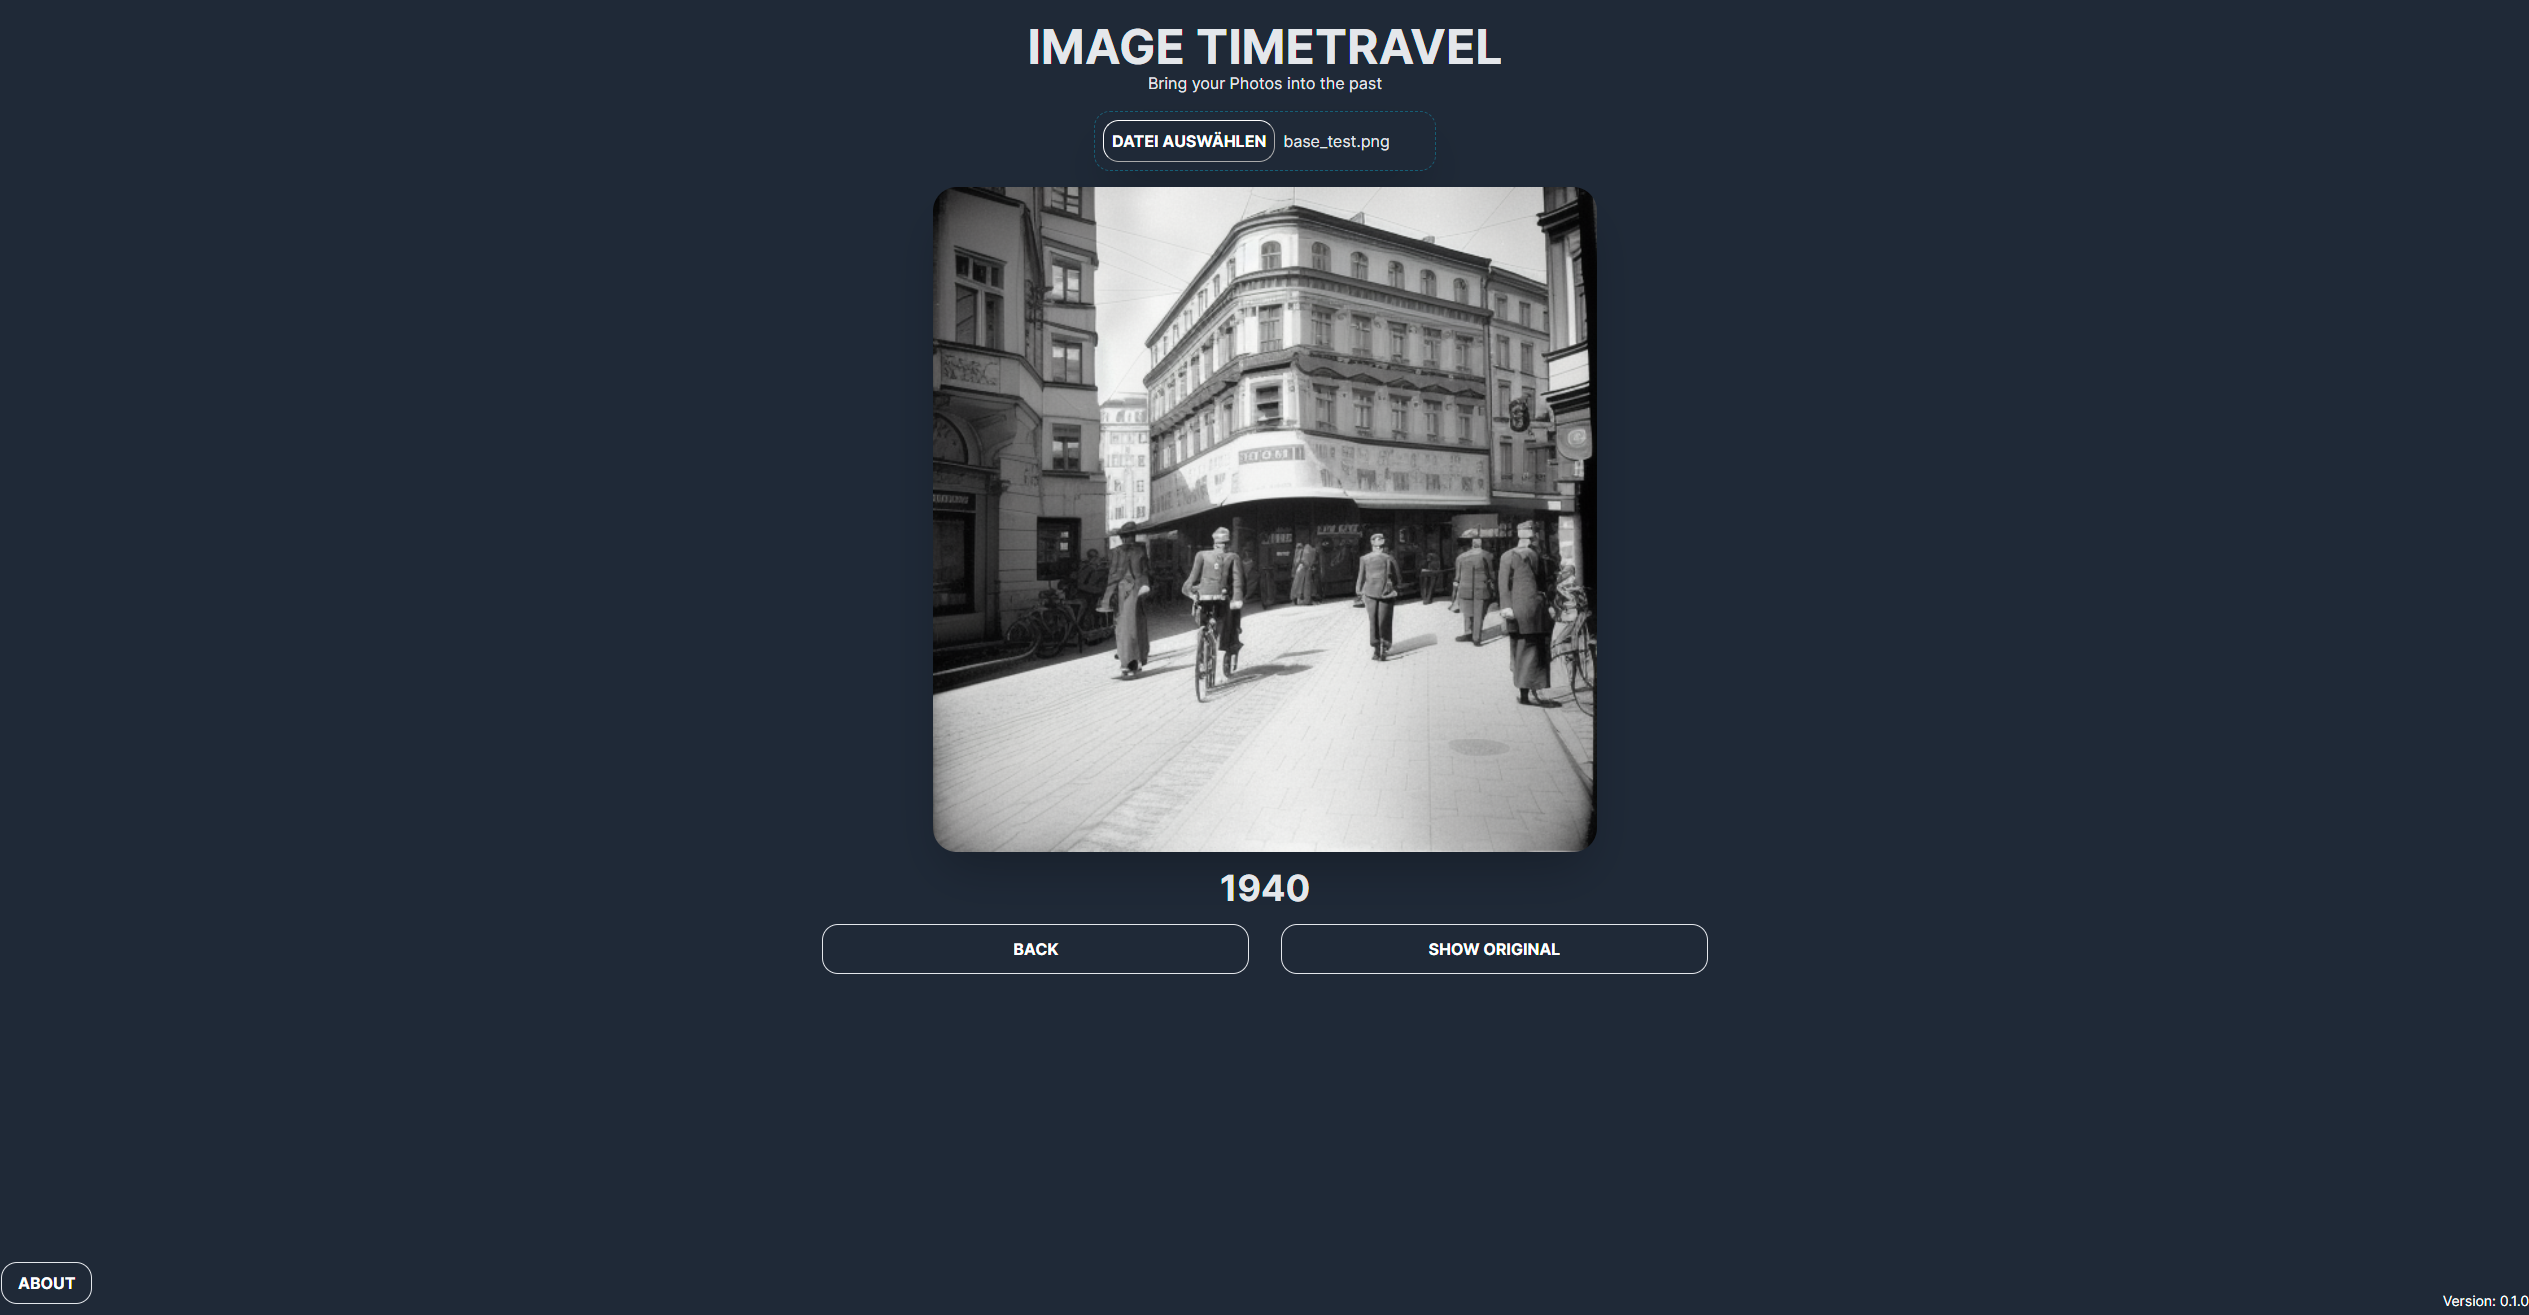
\includegraphics[width=0.8\textwidth]{images/frontendPost.png}}
    \caption{A screenshot of the frontend after image generation. This shows as street in Salzburg, Austria in 1940 as generated by stable diffusion based on the previous input.}
    \label{fig:frontendPost}
\end{figure}

%%%-----------------------------------------------------------------------------
\chapter{System Documentation}
%%%-----------------------------------------------------------------------------
\label{systemDocu}
In this chapter each part of the image generation is explained in detail.

\section{Stable Diffusion Setup}
The stable diffusion webUI \cite{webui} is locally hosted on a machine so that it can be used to transform images. A couple of changes were made the UI to make it possible to generate past version of images.
The specific stable diffusion model used is realistic vision V2.0 \cite{realisticVision}, which is supposed to generate more realistic looking images compared to the base stable diffusion model included in the webUI.

In order to get the image conversion working properly, the ControlNet plugin \cite{controllNet} is used to enhance images further. With the help of ControlNet canny it is possible to trace the outlines of objects in images that are put into stable diffusion, thereby resulting in images which more closely resemble the original.
Furthermore, the following settings were changed inside the webUI:
\begin{enumerate}
    \item under ControlNet: Allow other script to control this extension
    \item under Interrogate Options: Increase the minimum and maximum description length 
    \item under Interrogate Options: skip inquire categories for artists, flavors, mediums and movements 
\end{enumerate}
These settings ensure that ControlNet can be called from the frontend. Also, the changes to the interrogate options are vital, as otherwise the generated prompt for the past image could contain information about artists or non camera mediums which more often than not results in the generated image looking like a painting instead of a realistic photograph.

Finally, the command line section of the webui-user.bat file inside the folder for the stable diffusion webUI was changed to allow for API calls from the locally hosted front end as can be seen in the following code:

\begin{verbatim}
    set COMMANDLINE_ARGS= --xformers --autolaunch --medvram --api 
    --cors-allow-origins=http://127.0.0.1:7860 
    --cors-allow-origins=http://localhost:3000
\end{verbatim}

\section{The Frontend}
The frontend was developed using React, Typescript and NextJS 13. Therefore the project has the standard nextJS structure. The "app" folder contain the base layout of a page as well as all API routes. The "components" folder contains all components used on the pages. For styling purposes TailwindCSS was used. Since the frontend only serves as a UI for easier interaction and access to stable diffusion it was developed as a single page application.

\subsection{Components}
A total of three components were developed. \begin{itemize}
    \item BottomBar 
    \item TopNavigationBar
    \item FileUploader
\end{itemize}
The first two components are simply for cosmetic purposes while the FileUploader contains most of the logic.
\subsubsection{FileUploader}
The FileUploader has multiple state variables as well as function for executing the image conversion. Depending on its current states the FileUploader displays different parts. For example the year slider will only display after an image has been uploaded. The different state of the FileUploader can be seen here \ref{fig:FileUploaderStates}.

\begin{figure}[htbp]
    \centering\small
    \begin{tabular}{cc}
        \cr(On application start) & (After Image Upload)\\ 
        \fbox{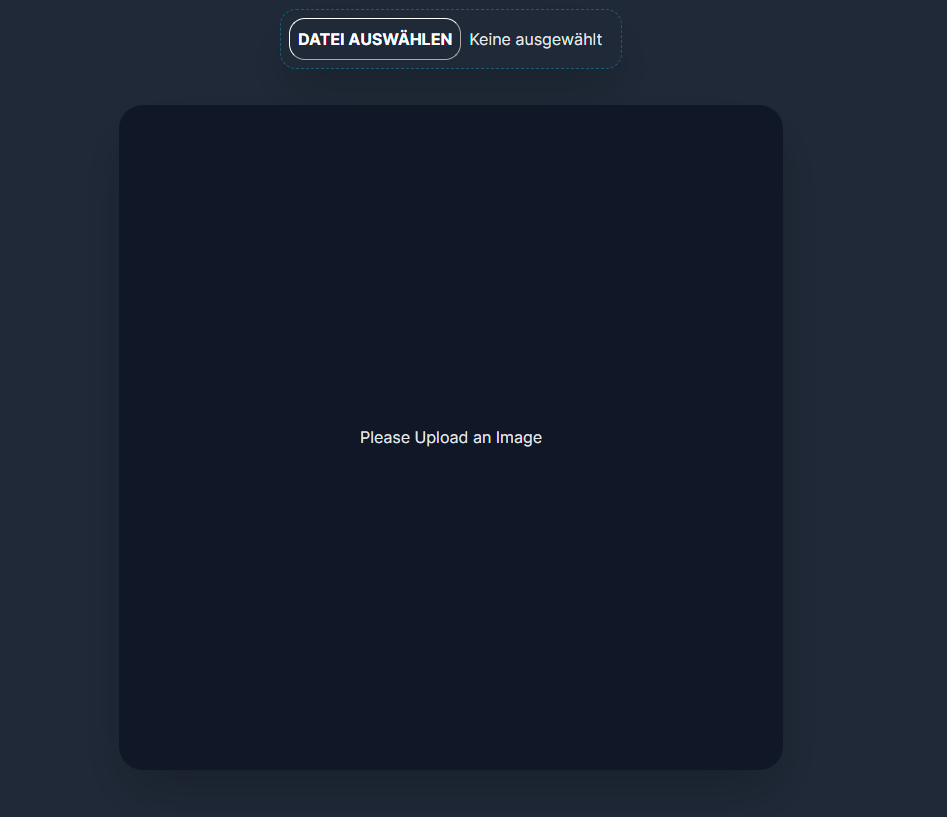
\includegraphics[width=0.45\textwidth]{images/FileUploaderEmpty.png}} & 
        \fbox{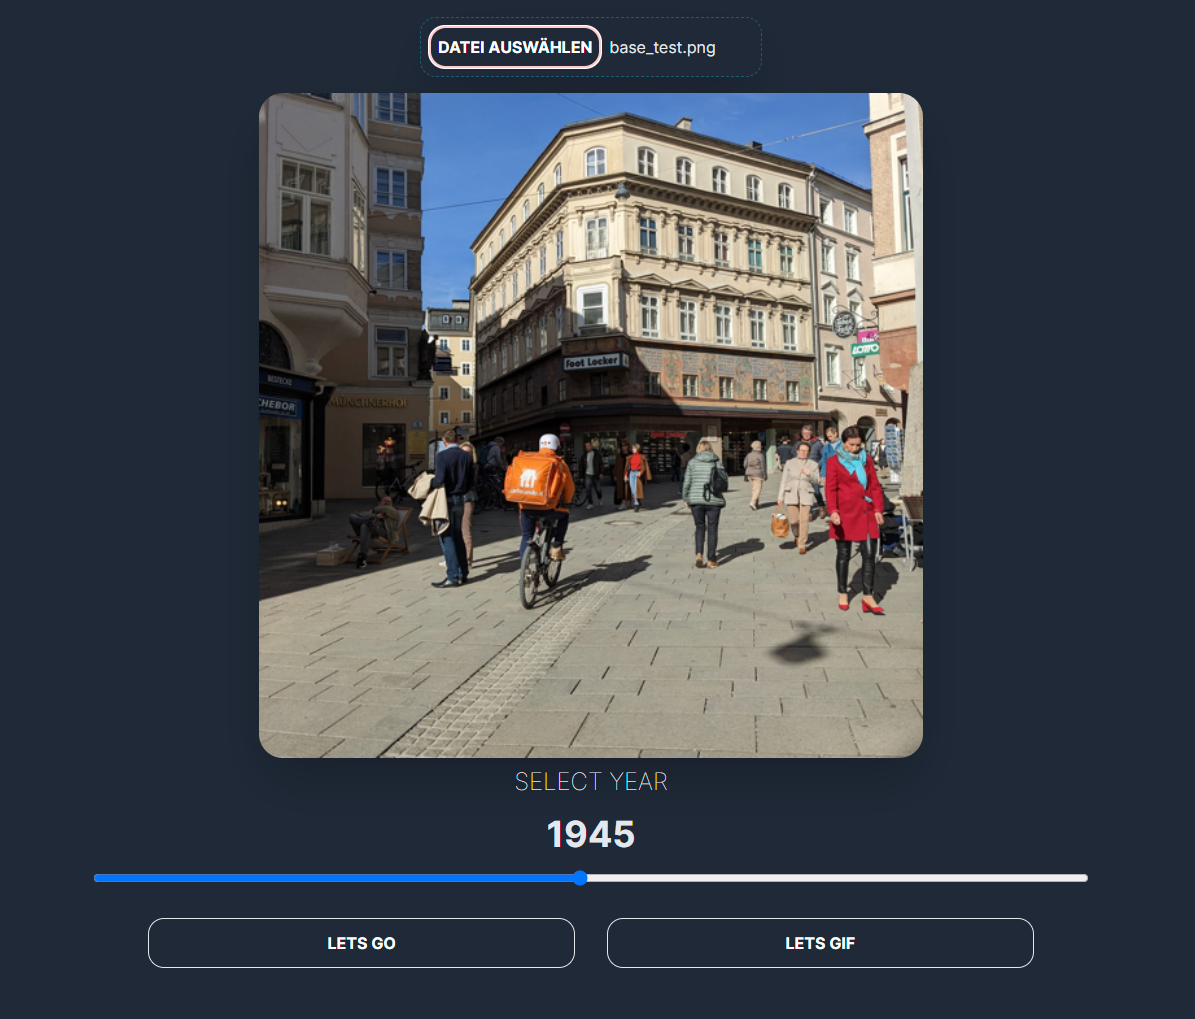
\includegraphics[width=0.45\textwidth]{images/FileUploaderEmpty_Image.png}}\\
        \cr(During image generation) & (Finished image conversion)\\
        \fbox{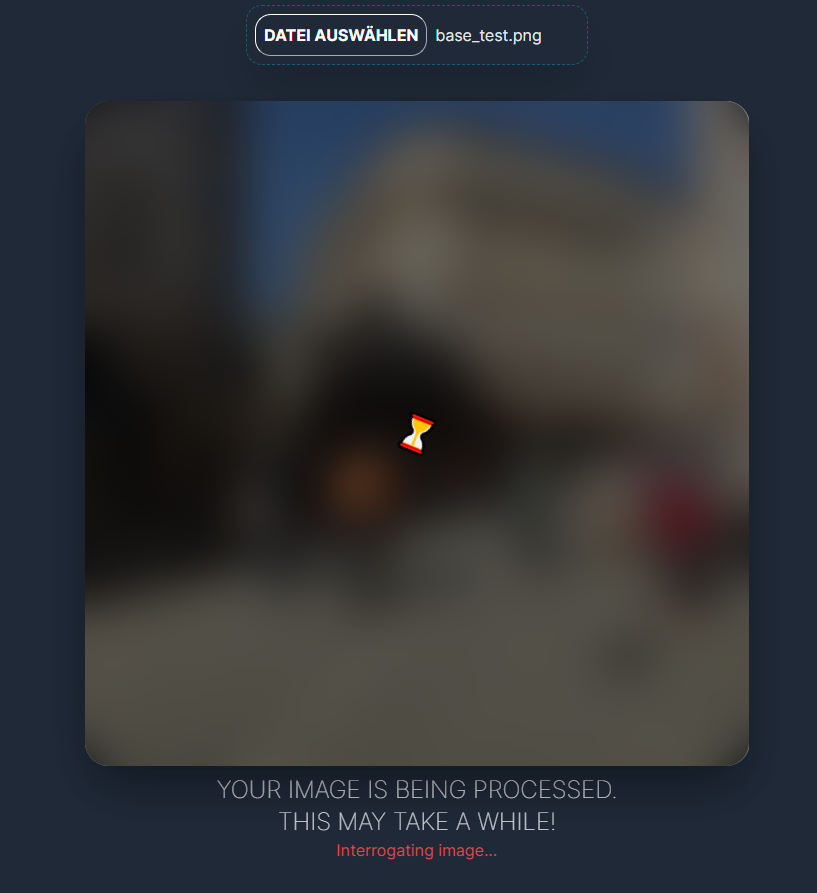
\includegraphics[width=0.45\textwidth]{images/FileUploaderEmpty_Loading.png}} & 
        \fbox{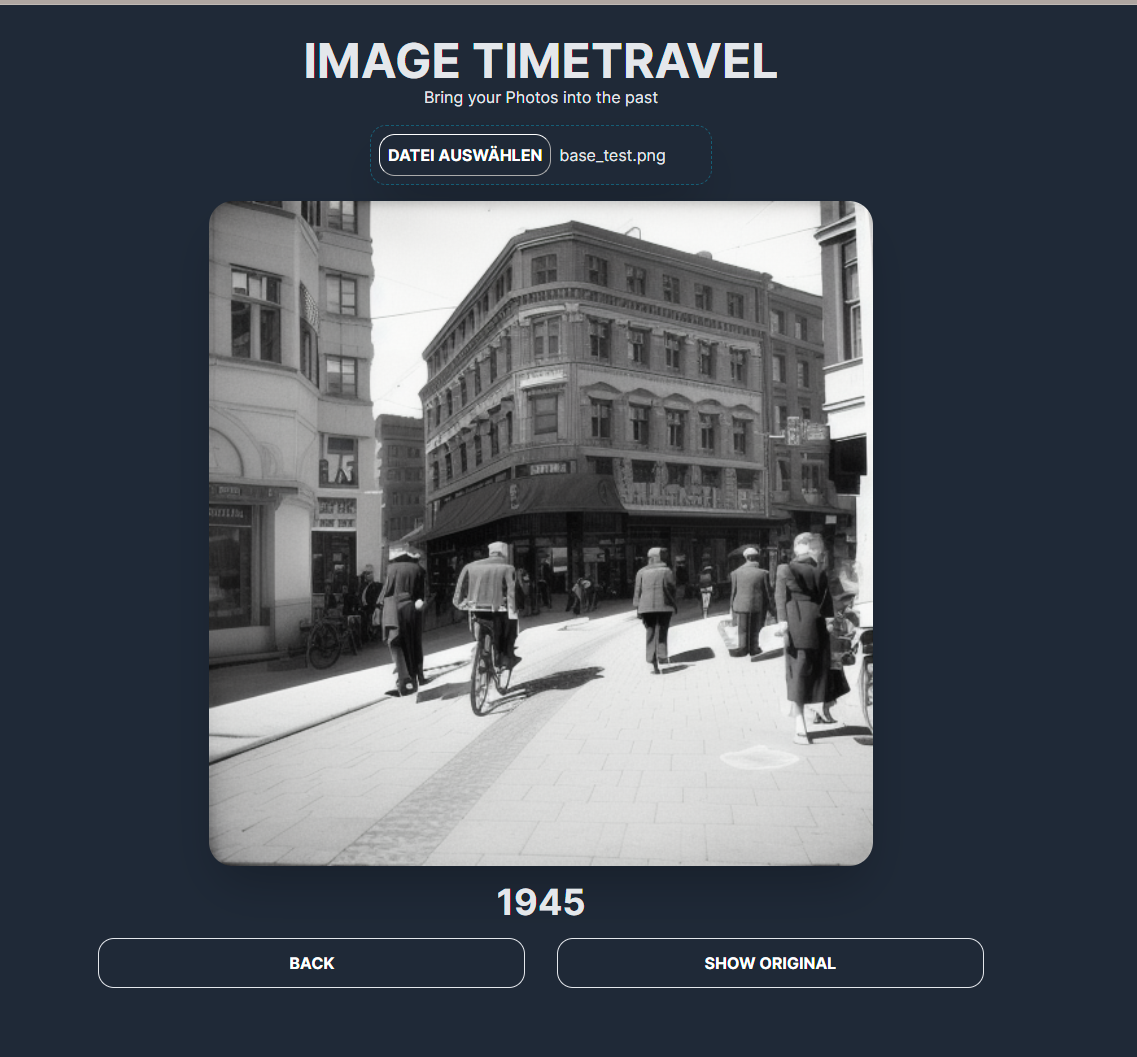
\includegraphics[width=0.52\textwidth]{images/FileUploaderEmpty_Finished.png}}
    \end{tabular}
    \caption{Screenshots of the FileUploader component during its different states.} 
    \label{fig:FileUploaderStates}
\end{figure}

The various functions used in the component are as follows: \begin{itemize}
    \item \textbf{handleFileSelect:} executed when an image is uploaded. Checks the file size and type of the uploaded image and then resizes it to 512x512 as well as read the geolocation data from the image.
    \item \textbf{cropImage:} a helper function used in handleFileSelect to properly crop the uploaded image.
    \item \textbf{getCityAndCountry:} a helper function used in handleFileSelect that makes an axios call to openstreetmap based on the latitude and longitude contained in the image geo location data in order to determine the city and country the image is from.
    \item \textbf{handleBackButton:} executes when the back button is pressed. Resets the state of the FileUploader to its initial state.
    \item \textbf{handleShowOriginalButton:} executes when the show original button is pressed. Swaps the currently displayed image with the original uploaded image and vice versa.
    \item \textbf{handleClick:} executes when the "Let´s Go" button is pressed. Calls each API route, as described in the next section \ref{apiRoutes}, after each other to generate a past version of the uploaded image.
    \item \textbf{handleClickGif:} executes when the "Let´s Gif" button is pressed. Functions the same way as handleClick but generates multiple images with the year starting at 1880 up to 2013 in five year increments instead. The generated images are then combined into a GIF. This function does not use the getGPT API route.
    \item \textbf{generateGif:} a helper function used in handleClickGif to combine the generated images into a GIF using gifjs.3
    \item \textbf{handleResponseImageClick:} executes when the generated image is clicked. Opens the image as a pop up.
\end{itemize}


\subsection{API Routes}
\label{apiRoutes}
A total of five API routes were implemented in order to have a cleaner code structure as well as keep server side code out of the FileUploader component.
\subsubsection{interrogateImage}
The first API route is interrogateImage which makes an API call to the locally hosted stable diffusion implementation and returns the generated image description.
\subsubsection{getPrompt}
The getPrompt API route filters out all colors from the prompt and contains prewritten prompt parts to the base prompt depending on the year.
\subsubsection{getGPT}
The getGPT API route makes an API call to chatGPT containing the year and prompt and request chatGPT to generate a list of negative prompts filled with objects that are contained inside the prompt but did not exist in the selected year.
\subsubsection{getNegativePrompt}
The getNegativePrompt API rout add additional prewritten negative prompts based on the selected year.
\subsubsection{convertImage}
The convertImage API route makes an API call to the locally hosted stable diffusion implementation containing the generated prompt, negative prompts as well as the input image.

%%%-----------------------------------------------------------------------------
\chapter{Summary}
%%%-----------------------------------------------------------------------------

Over the course of the semester a pipeline for generating a version of an image based on a specific past year was created.
Based on this pipeline a front end application was developed which makes it possible to upload single images as well as select a specific year to generate a past version of the uploaded image based on the selected year.
Additionally, uploaded images can also be turned into GIFs to have a time lapse over a whole year range going from 1880 to 2013

\section{Possible Issues}
In the current implementation the FileUploader component currently contains the bulk of the code in the front end, thereby making it a very bloated component. This can make it hard to expand the functionality of the whole application. 
The current solution always has to be locally hosted which requires users to have the stable diffusion webUI running as well. Since the stable diffusion webUI requires a decent GPU to run properly this can be an issue when working on a less powerful device. Steps were taken to try to host the stable diffusion webUI on one of the render nodes at the FH Hagenberg, but this still requires users to be inside the WiFi network of the universtiy as well as having the frontend application running locally.


%%%-----------------------------------------------------------------------------
\appendix                                                   % Switch to appendix
%%%-----------------------------------------------------------------------------
\chapter{Image showcase}

A showcase of some of the best images generated with the time machine.
\begin{figure}[htbp]
    \centering\small
    \begin{tabular}{cc}
        \cr(Attnang Austria 2023) & (Attnang Austria 1949)\\ 
        \fbox{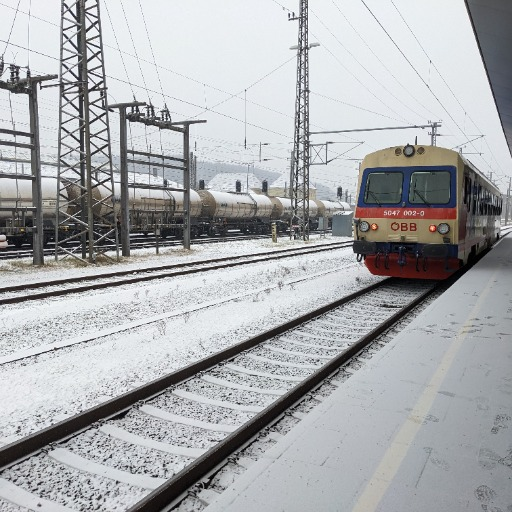
\includegraphics[width=0.45\textwidth]{images/best_of/attnang2023.jpg}} & 
        \fbox{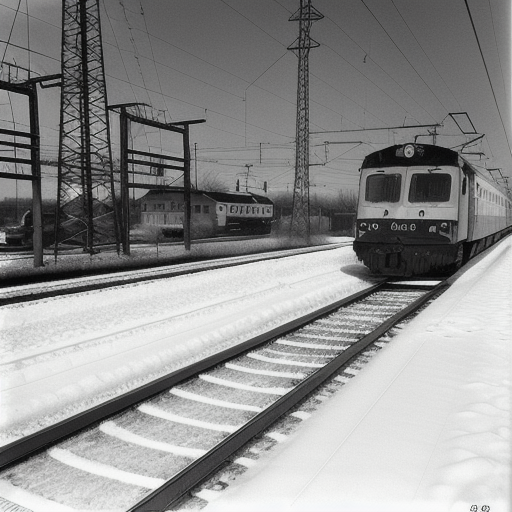
\includegraphics[width=0.45\textwidth]{images/best_of/attnang1949.png}}\\
    \end{tabular}
    \caption{Attnang Austria} 
\end{figure}
\begin{figure}[htbp]
    \centering\small
    \begin{tabular}{cc}
        \fbox{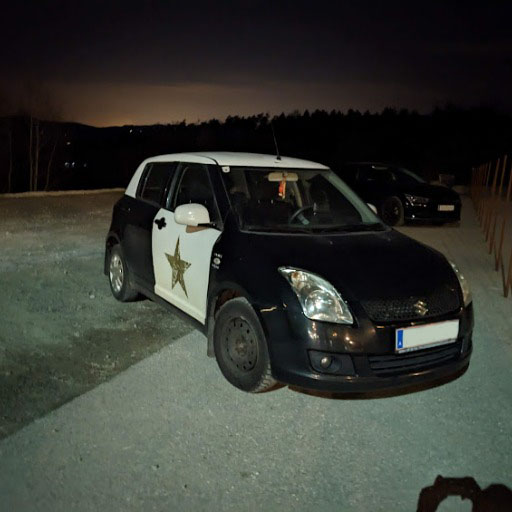
\includegraphics[width=0.45\textwidth]{images/best_of/bestof_car.jpg}} & 
        \fbox{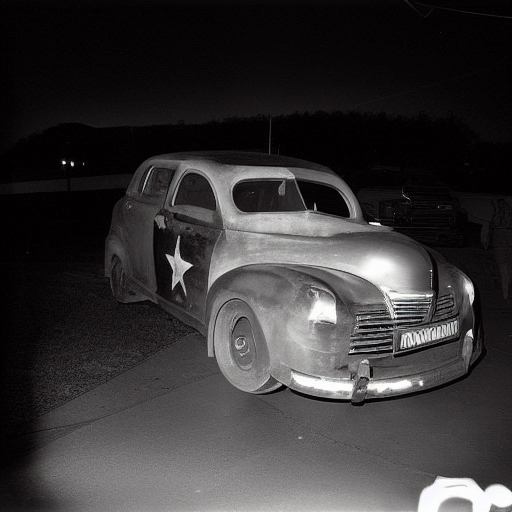
\includegraphics[width=0.45\textwidth]{images/best_of/bestof_carOld.png}}\\
    \end{tabular}
    \caption{A random car at one of the parking spots at the FH Hagenberg} 
\end{figure}
\begin{figure}[htbp]
    \centering\small
    \begin{tabular}{cc}
        \cr(Hamburg Germany 2018) & (Hamburg Germany 1945)\\ 
        \fbox{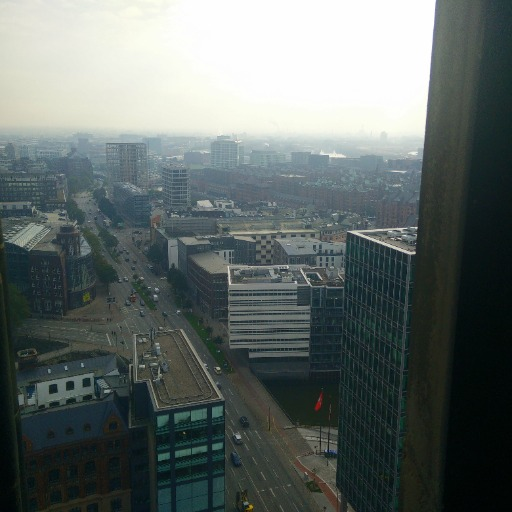
\includegraphics[width=0.45\textwidth]{images/best_of/hamburg2018.jpg}} & 
        \fbox{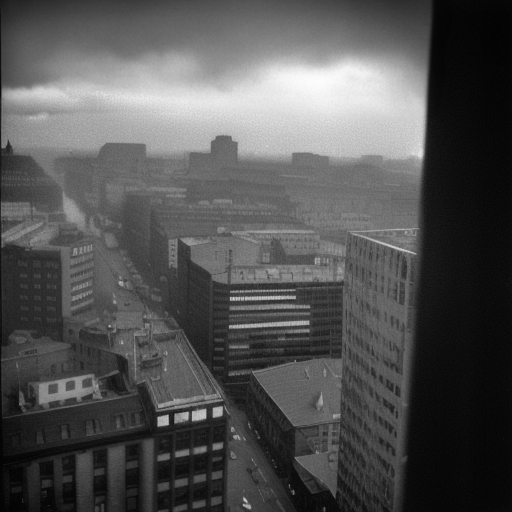
\includegraphics[width=0.45\textwidth]{images/best_of/hamburg1945.png}}\\
    \end{tabular}
    \caption{Hamburg Germany} 
\end{figure}
\begin{figure}[htbp]
    \centering\small
    \begin{tabular}{cc}
        \cr(Salzkammergut Austria 2023) & (Salzkammergut Austria 1996)\\ 
        \fbox{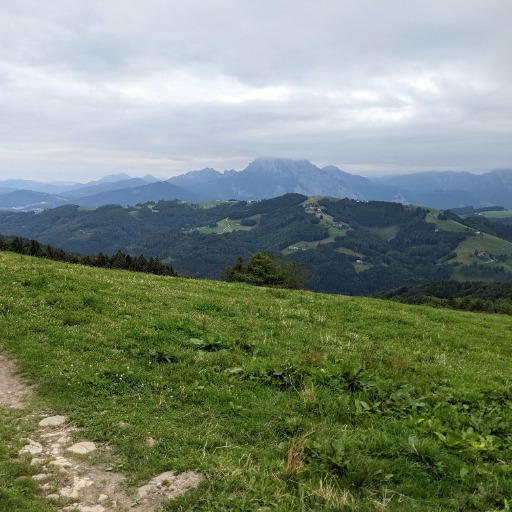
\includegraphics[width=0.45\textwidth]{images/best_of/Salzkammergut2023.jpg}} & 
        \fbox{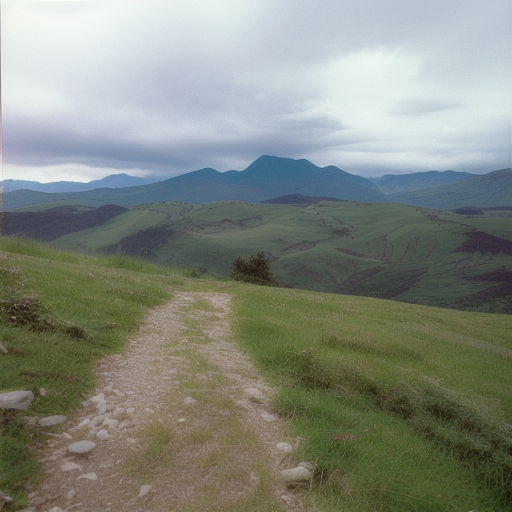
\includegraphics[width=0.45\textwidth]{images/best_of/Salzkamemrgut1996.png}}\\
    \end{tabular}
    \caption{Salzkammergut Austria} 
\end{figure}

%%%-----------------------------------------------------------------------------
\MakeBibliography[nosplit]
%%%-----------------------------------------------------------------------------

%%%-----------------------------------------------------------------------------
\end{document}
%%%-----------------------------------------------------------------------------
